% -*- Mode:TeX -*-

%% IMPORTANT: The official thesis specifications are available at:
%%            http://libraries.mit.edu/archives/thesis-specs/
%%
%%            Please verify your thesis' formatting and copyright
%%            assignment before submission.  If you notice any
%%            discrepancies between these templates and the 
%%            MIT Libraries' specs, please let us know
%%            by e-mailing thesis@mit.edu

%% The documentclass options along with the pagestyle can be used to generate
%% a technical report, a draft copy, or a regular thesis.  You may need to
%% re-specify the pagestyle after you \include  cover.tex.  For more
%% information, see the first few lines of mitthesis.cls. 

%\documentclass[12pt,vi,twoside]{mitthesis}
%%
%%  If you want your thesis copyright to you instead of MIT, use the
%%  ``vi'' option, as above.
%%
%\documentclass[12pt,twoside,leftblank]{mitthesis}
%%
%% If you want blank pages before new chapters to be labelled ``This
%% Page Intentionally Left Blank'', use the ``leftblank'' option, as
%% above. 

\documentclass[12pt,twoside]{mitthesis}
\usepackage{lgrind}
%% These have been added at the request of the MIT Libraries, because
%% some PDF conversions mess up the ligatures.  -LB, 1/22/2014
\usepackage{cmap}
\usepackage[T1]{fontenc}
\pagestyle{plain}

%% This bit allows you to either specify only the files which you wish to
%% process, or `all' to process all files which you \include.
%% Krishna Sethuraman (1990).

% \typein [\files]{Enter file names to process, (chap1,chap2 ...), or `all' to
% process all files:}
% \def\all{all}
% \ifx\files\all \typeout{Including all files.} \else \typeout{Including only \files.} \includeonly{\files} \fi

\begin{document}

% -*-latex-*-
% 
% For questions, comments, concerns or complaints:
% thesis@mit.edu
% 
%
% $Log: cover.tex,v $
% Revision 1.8  2008/05/13 15:02:15  jdreed
% Degree month is June, not May.  Added note about prevdegrees.
% Arthur Smith's title updated
%
% Revision 1.7  2001/02/08 18:53:16  boojum
% changed some \newpages to \cleardoublepages
%
% Revision 1.6  1999/10/21 14:49:31  boojum
% changed comment referring to documentstyle
%
% Revision 1.5  1999/10/21 14:39:04  boojum
% *** empty log message ***
%
% Revision 1.4  1997/04/18  17:54:10  othomas
% added page numbers on abstract and cover, and made 1 abstract
% page the default rather than 2.  (anne hunter tells me this
% is the new institute standard.)
%
% Revision 1.4  1997/04/18  17:54:10  othomas
% added page numbers on abstract and cover, and made 1 abstract
% page the default rather than 2.  (anne hunter tells me this
% is the new institute standard.)
%
% Revision 1.3  93/05/17  17:06:29  starflt
% Added acknowledgements section (suggested by tompalka)
% 
% Revision 1.2  92/04/22  13:13:13  epeisach
% Fixes for 1991 course 6 requirements
% Phrase "and to grant others the right to do so" has been added to 
% permission clause
% Second copy of abstract is not counted as separate pages so numbering works
% out
% 
% Revision 1.1  92/04/22  13:08:20  epeisach

% NOTE:
% These templates make an effort to conform to the MIT Thesis specifications,
% however the specifications can change.  We recommend that you verify the
% layout of your title page with your thesis advisor and/or the MIT 
% Libraries before printing your final copy.
\title{TaleBlazer Analytics: Automated Anonymous Analytics of Mobile Users' Behavior}

\author{Fidel Sosa}
% If you wish to list your previous degrees on the cover page, use the 
% previous degrees command:
%       \prevdegrees{A.A., Harvard University (1985)}
% You can use the \\ command to list multiple previous degrees
%       \prevdegrees{B.S., University of California (1978) \\
%                    S.M., Massachusetts Institute of Technology (1981)}
\prevdegrees{S.B, Massachusetts Institute of Technology, (2011)}
\department{Department of Electrical Engineering and Computer Science}

% If the thesis is for two degrees simultaneously, list them both
% separated by \and like this:
% \degree{Doctor of Philosophy \and Master of Science}
\degree{Master of Engineering in Computer Science and Engineering}

% As of the 2007-08 academic year, valid degree months are September, 
% February, or June.  The default is June.
\degreemonth{June}
\degreeyear{2014}
\thesisdate{May 23, 2014}

%% By default, the thesis will be copyrighted to MIT.  If you need to copyright
%% the thesis to yourself, just specify the `vi' documentclass option.  If for
%% some reason you want to exactly specify the copyright notice text, you can
%% use the \copyrightnoticetext command.  
%\copyrightnoticetext{\copyright IBM, 1990.  Do not open till Xmas.}

% If there is more than one supervisor, use the \supervisor command
% once for each.
\supervisor{Professor Eric Klopfer}{Director, MIT Scheller Teacher Education Program}

% This is the department committee chairman, not the thesis committee
% chairman.  You should replace this with your Department's Committee
% Chairman.
\chairman{Prof. Albert R. Meyer}{Chairman, Masters of Engineering Thesis Committee}

% Make the titlepage based on the above information.  If you need
% something special and can't use the standard form, you can specify
% the exact text of the titlepage yourself.  Put it in a titlepage
% environment and leave blank lines where you want vertical space.
% The spaces will be adjusted to fill the entire page.  The dotted
% lines for the signatures are made with the \signature command.
\maketitle

% The abstractpage environment sets up everything on the page except
% the text itself.  The title and other header material are put at the
% top of the page, and the supervisors are listed at the bottom.  A
% new page is begun both before and after.  Of course, an abstract may
% be more than one page itself.  If you need more control over the
% format of the page, you can use the abstract environment, which puts
% the word "Abstract" at the beginning and single spaces its text.

%% You can either \input (*not* \include) your abstract file, or you can put
%% the text of the abstract directly between the \begin{abstractpage} and
%% \end{abstractpage} commands.

% First copy: start a new page, and save the page number.
\cleardoublepage
% Uncomment the next line if you do NOT want a page number on your
% abstract and acknowledgments pages.
% \pagestyle{empty}
\setcounter{savepage}{\thepage}
\begin{abstractpage}
% $Log: abstract.tex,v $
% Revision 1.1  93/05/14  14:56:25  starflt
% Initial revision
% 
% Revision 1.1  90/05/04  10:41:01  lwvanels
% Initial revision
% 
%
%% The text of your abstract and nothing else (other than comments) goes here.
%% It will be single-spaced and the rest of the text that is supposed to go on
%% the abstract page will be generated by the abstractpage environment.  This
%% file should be \input (not \include 'd) from cover.tex.
TaleBlazer is an augmented-reality platform that lets users create location-based games for their mobile devices. In order to determine the efficacy and use cases for TaleBlazer games, it is necessary to capture data about user behavior. This thesis presents TaleBlazer Analytics, an automated system which collects and analyzes mobile users' behavior in TaleBlazer games. It details the development of the TaleBlazer Analytics system, comprised of the backend data collection service and the front-end data analysis user interface. 

 

\end{abstractpage}

% Additional copy: start a new page, and reset the page number.  This way,
% the second copy of the abstract is not counted as separate pages.
% Uncomment the next 6 lines if you need two copies of the abstract
% page.
% \setcounter{page}{\thesavepage}
% \begin{abstractpage}
% % $Log: abstract.tex,v $
% Revision 1.1  93/05/14  14:56:25  starflt
% Initial revision
% 
% Revision 1.1  90/05/04  10:41:01  lwvanels
% Initial revision
% 
%
%% The text of your abstract and nothing else (other than comments) goes here.
%% It will be single-spaced and the rest of the text that is supposed to go on
%% the abstract page will be generated by the abstractpage environment.  This
%% file should be \input (not \include 'd) from cover.tex.
TaleBlazer is an augmented-reality platform that lets users create location-based games for their mobile devices. In order to determine the efficacy and use cases for TaleBlazer games, it is necessary to capture data about user behavior. This thesis presents TaleBlazer Analytics, an automated system which collects and analyzes mobile users' behavior in TaleBlazer games. It details the development of the TaleBlazer Analytics system, comprised of the backend data collection service and the front-end data analysis user interface. 

 

% \end{abstractpage}

\cleardoublepage

\section*{Acknowledgments}

I'd like to thank Eric Kloper, Lisa Stump, and Judy Perry for giving me the opportunity to work on this project. It has been an eye-opening and rewarding experience that would not be possible without them. 

I'd like to thank Lisa Stump for being a guiding force and great help during the project, as well as helping me determine a set of achievable goals for the project. I'd also like to thank Judy Perry for all the guidance and management she provided. This project would not have been as successful as it was without them. 

I'd also like to thank the entire TaleBlazer Development team, including my fellow M.Engs Tanya Liu, Cristina Lozano, and Stephanie Chang. They provided much help in testing and making this project fun to work on.

I'd like to thank my academic supervisor, Boris Katz. Without his help during my undergraduate and graduate years, I would not be where I currently am. A great thanks to my friends, as well, who have supported me throughout the years. 

Finally, I'd like to thank my family, whose sacrifices have allowed me to be where I am today.  

%%%%%%%%%%%%%%%%%%%%%%%%%%%%%%%%%%%%%%%%%%%%%%%%%%%%%%%%%%%%%%%%%%%%%%
% -*-latex-*-

% Some departments (e.g. 5) require an additional signature page.  See
% signature.tex for more information and uncomment the following line if
% applicable.
% % -*- Mode:TeX -*-
%
% Some departments (e.g. Chemistry) require an additional cover page
% with signatures of the thesis committee.  Please check with your
% thesis advisor or other appropriate person to determine if such a 
% page is required for your thesis.  
%
% If you choose not to use the "titlepage" environment, a \newpage
% commands, and several \vspace{\fill} commands may be necessary to
% achieve the required spacing.  The \signature command is defined in
% the "mitthesis" class
%
% The following sample appears courtesy of Ben Kaduk <kaduk@mit.edu> and
% was used in his June 2012 doctoral thesis in Chemistry. 

\begin{titlepage}
\begin{large}
This doctoral thesis has been examined by a Committee of the Department
of Chemistry as follows:

\signature{Professor Jianshu Cao}{Chairman, Thesis Committee \\
   Professor of Chemistry}

\signature{Professor Troy Van Voorhis}{Thesis Supervisor \\
   Associate Professor of Chemistry}

\signature{Professor Robert W. Field}{Member, Thesis Committee \\
   Haslam and Dewey Professor of Chemistry}
\end{large}
\end{titlepage}


\pagestyle{plain}
  % -*- Mode:TeX -*-
%% This file simply contains the commands that actually generate the table of
%% contents and lists of figures and tables.  You can omit any or all of
%% these files by simply taking out the appropriate command.  For more
%% information on these files, see appendix C.3.3 of the LaTeX manual. 
\tableofcontents
\newpage
\listoffigures
\newpage
\listoftables
\newpage
\lstlistoflistings


%!TEX root = main.tex
\chapter{Introduction}

The explosion of the mobile market has led to the proliferation of location-aware mobile devices and a wide range of mobile applications (``apps'') that provide location-based content. Augmented reality (AR) applications, for example, enhance the user's real-life environment with location-specific information. The prevalence and affordability of these mobile devices, such as smartphones and tablets, make them a natural choice as a tool to augment education and learning. TaleBlazer is an augmented reality location-based games platform that allows users to create their own games that take place in the real world and play them on their mobile devices. A goal of the TaleBlazer project is to determine the education impact of location-based games. TaleBlazer Analytics is an automated system that allows game designers and researchers to gather and analyze anonymous data about users' behaviors during TaleBlazer games. 

\section{Motivations for TaleBlazer Analytics}
The wide gamut of user-created TaleBlazer games requires a data collection system that is both flexible and useful. TaleBlazer Analytics was developed to allow game designers and researchers to get specific metrics about when and how their games are played. For game designers, these metrics allow them to create more engaging and effective game experiences. For researchers, these metrics provide crucial information such as how players progress through the game and the choices that they make. Past data collection, game designers and researchers also need a way to quickly analyze the vast amount of gameplay data that is generated. 

Existing analytics solutions fail to provide data analytics useful to TaleBlazer specifically and often do not provide an adequate level of user privacy. Furthermore, the unique nature of TaleBlazer games requires custom analysis of the generated data. As a result, it was necessary to develop TaleBlazer Analytics to meet our needs. 

Over the past year and a half, I have developed an automated data collection system which seamlessly integrates with the existing TaleBlazer app and server architecture, working closely at each step with the TaleBlazer team. TaleBlazer Analytics is comprised of a backend server, mobile client, and web application, jointly responsible for the collection, storage, and analysis of TaleBlazer gameplay data. 

\section{Chapter Summary}
This thesis describes the background, design, and development of the TaleBlazer Analytics system. Chapter 2 details TaleBlazer in-depth and expands on the need for TaleBlazer Analytics. Chapter 3 explains the design process and preliminary decisions required for the development of TaleBlazer Analytics. Chapters 4, 5, 6, 7 detail the server, client, and web applications components of the project. Chapter 8 discusses the process of user testing and feedback that we received. Chapter 9 proposes future work for the project and Chapter 10 provides parting thoughts. 





%!TEX root = main.tex
\chapter{Background}

This chapter gives a background on the TaleBlazer project, including its separate components and how they work together as a whole. The history of TaleBlazer and past location-based projects are also detailed. Finally, the chapter expands on the need for TaleBlazer Analytics.

\section{TaleBlazer}

TaleBlazer is an augmented reality location-based game platform developed at the MIT Scheller Teacher Education Program (STEP). TaleBlazer is a platform in the true sense in that it is composed of multiple technologies which all come together to produce the TaleBlazer experience. At its core, TaleBlazer lets users create their own games that take place in the real world, using a web-based game editor. Users can then choose to publish their games to the world at large. Using the Android or iOS TaleBlazer mobile application, players play TaleBlazer games by downloading the game and physically walking around in the real-world location that the game takes place in. Players interact with with virtual game agents: user-scripted  entities that are placed by the game designer at specific GPS coordinates.

\subsection{Overview of a TaleBlazer Game}

A typical TaleBlazer game consists of the following parts: 
	\begin{itemize}
		\item regions, which are the real-world locations where the game takes place
		\item roles, which encompass different sets of behaviors for the player(s) in the game
		\item scenarios, which encompass different versions of a game
		\item agents, which are in-game virtual entities that player(s) interact with
		\item traits, variables that belong to different in-game entities or the world
		\item scriptblocks, sets of programming instructions that define the behaviors for game entities
	\end{itemize}

\subsubsection{Regions}

Regions are real-world locations where TaleBlazer games take place. Using the game editor, game designers define their game regions by selecting an area of a Google map. Regions define the area where in-game virtual entities, called agents, can be placed. Games can have one or more regions, each with their own name. The game designer also has the option of moving the player or agents from one region to another during the course of game using TaleBalzer's programming language. In order to play a TaleBlazer game, a player goes to the real-world location with their mobile device and moves around the region to activate or ``bump'' into the agents placed at nearby locations. 

\subsubsection{Roles}

Roles allow game designers to define different characters or types of interactions for different sets of players. This allows designers to create role-playing game experiences. A game can have one or more roles. If a single role is defined, then all players experience the same game. Multiple roles let the game designer define different sets of behaviors for different roles. Each role has a name and an optional description, which players see when choosing between roles at the start of a TaleBlazer game. For example, a game might have players choose between the roles of ``Secret Agent'' and ``Police Officer''.

\subsubsection{Scenarios}

Scenarios allow game designers to create different versions of the same game that players can choose between. For example, scenarios could be difficulty options, such as ``Easy'', ``Medium'', and ``Hard''. Games can have one or more scenarios, each with their own name. If a game has multiple scenarios, then the player is asked to choose between them at the start of a game. The game designer can tailor the behaviors of his game according to the choice of scenario. 

\subsubsection{Agents}

Agents are the in-game virtual entities with which players interact during the course of a TaleBlazer game. Agents have a name, description, set of behaviors, and an optional real-world location. Agents could be anything from items like a treasure chest to a non-player character (NPC) that gives a player quests. Users have multiple methods by which they can interact with agents. Agents placed within a region have corresponding GPS coordinates. Players interact with the agent by arriving at the GPS coordinates of an agent. Some games allow the user to tap on an agent's icon on the map of the game to interact with the agent, referred to as ``tap-to-visit''. Although there are many different ways that a player could come to interact with an agent, an agent interaction in general is referred to as an agent bump.

\subsubsection{Traits}

Traits are variables that can be attached to agents, roles, or the game world in general. Traits have names and values and can be modified during the course of a game based on the behaviors defined by the game designer. Game designers can create their own custom traits, each with a user-defined value. Traits can be used to represent game mechanics, such as a score.

\subsubsection{ScriptBlocks}

ScriptBlocks is a block-based programming language that allows game designers to define the behaviors for their game. ScriptBlocks is block-based because all programming instructions come in the form of blocks that you connect together using a visual game editor (see Figure \ref{fig:game_editor}). For example, conditional behaviors can be defined using a conditional IF-ELSE block, which has sockets that allow you to insert other blocks to define the conditional statement to evaluate. Game designers can write game behaviors by creating agent or role-specific scripts, or by writing scripts applicable to the entire game world. 

TaleBlazer contains a comprehensive set of programming blocks, encompassing a variety of purposes from logical and mathematical functions to TaleBlazer-specific commands. For example, a user can easily check the state of a game agent or move an agent or player from one location to another.

\medskip
\begin{figure}[hbt]
	\center{
			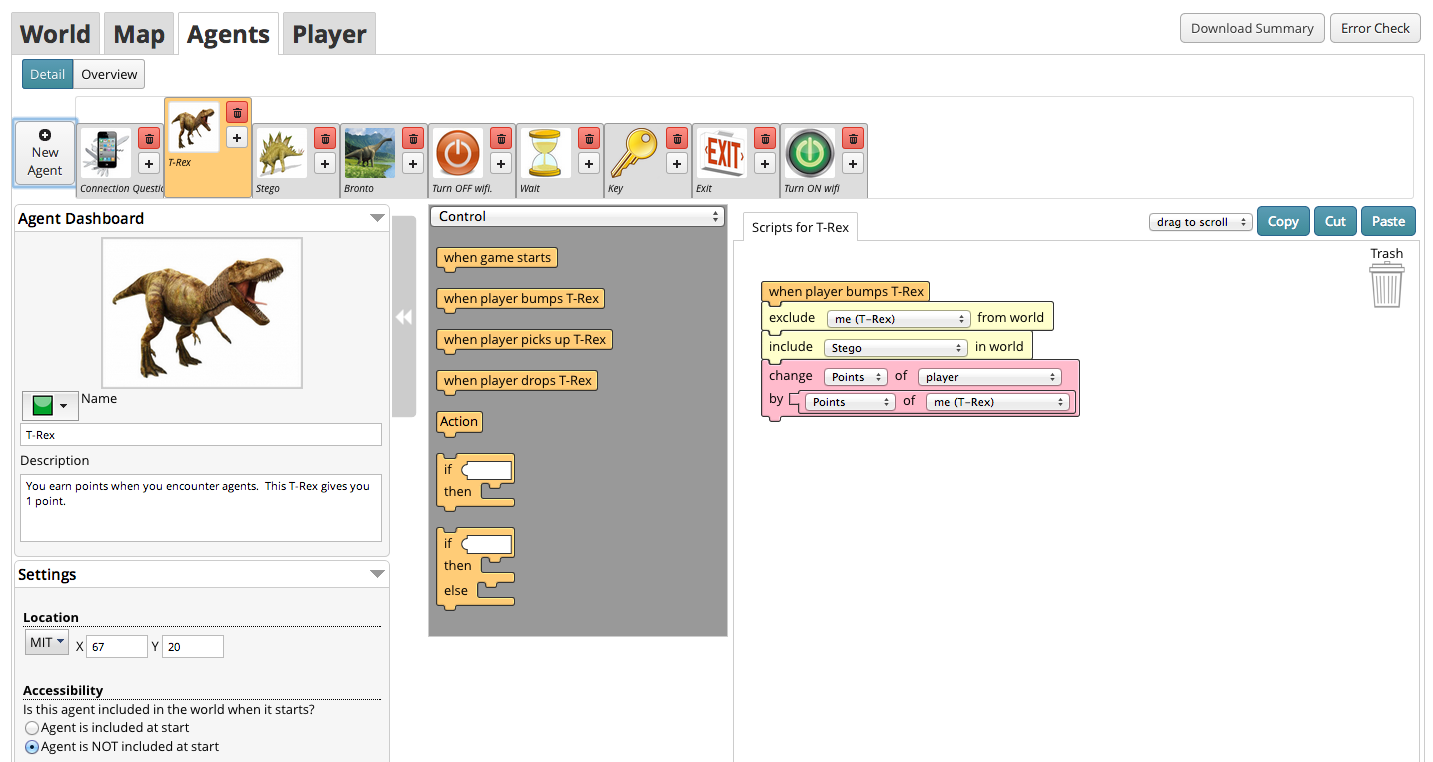
\includegraphics[width=\textwidth]
				{figures/game_editor.png}
			}
	\caption[TaleBlazer Game Editor]{\label{fig:game_editor} The TaleBlazer Game Editor web application}
\end{figure}
\pagebreak

\subsection{TaleBlazer Technology}

The TaleBlazer platform is comprised of four main parts:
	\begin{itemize}
 		\item the game editor, which lets users create their own games
 		\item the mobile application, on which TaleBlazer games are played
 		\item the repository server, which stores and serves games
 		\item and the multiplayer server, which enables multiplayer TaleBlazer games
 	\end{itemize}

\subsubsection{Game Editor}
The game editor is an online web application which lets users create their own TaleBlazer games through the use of ScriptBlocks. Using the editor, users add and configure their game regions, create agents, roles and scenarios, and program the game by composing scripts. Users can save their games, which are then stored on TaleBlazer Server. The game editor also provides options for modifying the game interface that players see when playing a game on their mobile device. The game editor is written in JavaScript. 

\subsubsection{TaleBlazer Mobile}

TaleBlazer Mobile is an Android and iOS mobile application that lets users play TaleBlazer games. The app lets users download TaleBlazer games onto their device and play them, utilizing the location-aware functionalities of the device. TaleBlazer Mobile interprets the blocks in each game file and executes them during the course of the game.

The TaleBlazer Mobile game interface consists primarily of a map of the current game region and icons indicating the position of the player and active game agents (see Figure \ref{fig:app_ui}). Tabs along the top of the screen provide different gameplay functionalities. For example, a game can include the Inventory tab, which tracks currently held items, or the Log tab, which contains a log of all the actions a player has taken during the course of a game.

TaleBlazer Mobile is written using Appcelerator Titanium, an SDK that lets developer write native Android and iOS applications using JavaScript. 

\medskip
\begin{figure}[htb]
	\center{
			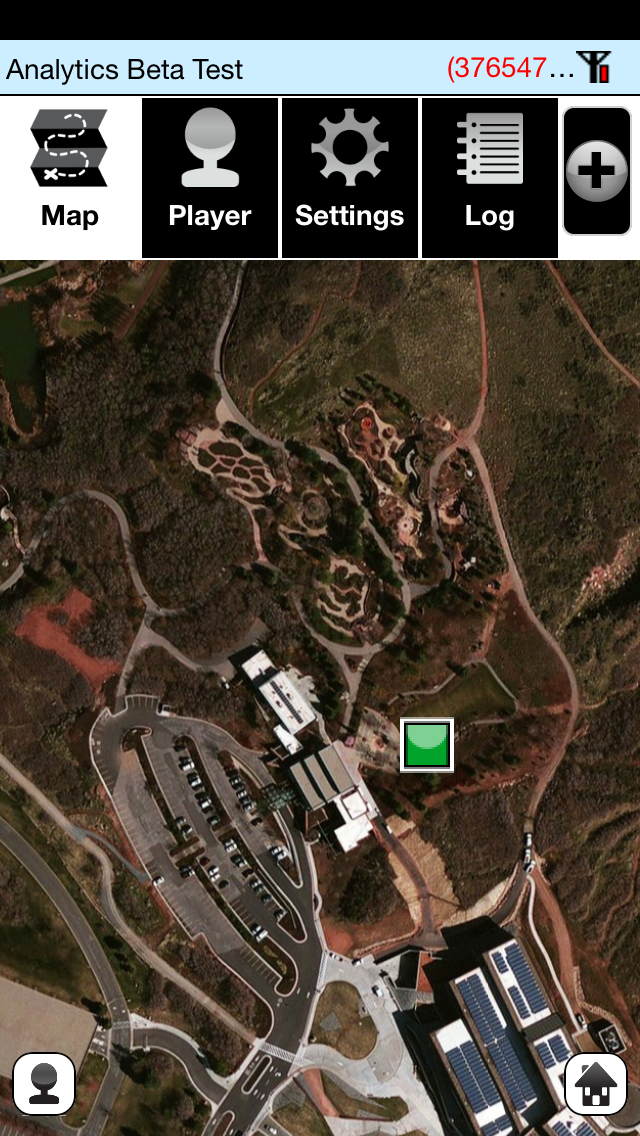
\includegraphics[scale=0.3]
				{figures/app_ui.png}
			}
	\caption[TaleBlazer Mobile Map UI]{\label{fig:app_ui} The TaleBlazer Mobile Main Map Interface}
\end{figure}

\subsubsection{TaleBlazer Server}

TaleBlazer Server is the main repository server which handles user accounts, hosts the game editor, and stores and serves TaleBlazer games and game-related files (e.g. images, video). TaleBlazer Server is written in PHP using the CakePHP framework and backed by a MySQL database. 

\subsubsection{TaleBlazer Multiplayer}

TaleBlazer Multiplayer is a separate server which provides multiplayer functionality for TaleBlazer games. It implements a separate protocol which synchronizes the state of the world between all devices playing a multiplayer game. The server is written in Node.js, using JavaScript.

\subsection{Past Projects}

TaleBlazer is the most recent iteration and study into AR games performed at the STEP lab. Past projects, such as MITAR and StarLogo TNG, provided a basis on which TaleBlazer was built, namely the emphasis on augmented reality and the use of a block-based scripting language.

\subsubsection{MITAR}

MITAR (MIT Augmented Reality) was the immediate ancestor of TaleBlazer. Similar to TaleBlazer, MITAR sought to let users play location-based augmented reality games on earlier mobile platforms, such as Windows Mobile. MITAR also focused on the educational impact of augmented reality games on users. One game, called ``Environmental Detectives'', put users into the roles of investigators searching for the source of a toxic spill, taking measurements in order to determine the environmental impact. \cite{site:ed}

\subsubsection{StarLogo TNG}

StarLogo TNG (The Next Generation) was a project in programmable simulation modeling which allowed users to explore the workings of complex decentralized systems, such as ant colonies and traffic jams. \cite{site:starlogo} Similar to TaleBlazer, users could program the simulation using a block-based scripting language. 

\section{Why Build TaleBlazer Analytics?}

The educational focus of the TaleBlazer project requires that the impact of TaleBlazer games on learning be measured. Game designers and educational researchers are supremely interested in seeing exactly how players play their games in order to draw conclusions as to their games' success and impact.

The rationale behind building TaleBlazer Analytics is two-fold. First, the public release of TaleBlazer requires an automated way of gathering quantitative data about all gameplay sessions. Previously, the only way to gather data was by observing players as they played. Second, existing analytics solutions fail to provide analytics relevant to TaleBlazer with a desirable level of privacy. To this end, it was necessary to build TaleBlazer Analytics to meet our requirements.

\subsection{Purpose of Data Collection}

The overall purpose of collecting TaleBlazer gameplay metrics is to provide interested parties with information to make informed decisions regarding the effectiveness of their game, across different aspects. Specifically, these parties are interested in quantitative metrics, such as the number of players that completed a game and the choices that were made during a gameplay session. 

This type of data could be used to identify buggy game scripts or points of player confusion. It could also be used to determine the appeal of specific narrative elements. For example, a game designer would be able to determine if changing the name of a role from ``Police Officer'' to ``Officer Awesome'' made the role more appealing.

There are four main parties that are interested in this type of data: 
	\begin{itemize}
		\item Game designers
		\item Educational researchers
		\item TaleBlazer developers
		\item Institutions
	\end{itemize}

\subsubsection{Game designers}
Game designers are primarily interested in seeing how players progress through the game and the choices they make along the way. Using this information, a game designer can quickly identify problematic spots. For example, players may stop playing after a particular point in the game because the instructions to proceed aren't clear or there is a bug in the game scripts. As a result, the game designer can improve the game to make it a better experience for the players.

\subsubsection{Educational researchers}

Educational researchers are interested in seeing how a game's content affects a player in the short or long-term. The choices that a player makes during a session can inform the researcher as to the level of a player's knowledge or how the content affected the player's understanding of the topic at hand. The gameplay metrics can be paired with external data, such as post-gameplay questionnaires or interviews. For example, a researcher studying a game about the environment might look at if a player encountered an EPA agent in-game or how fast they completed the game to see if a player missed crucial information or may not have been paying attention. Games can also include in-game research questions, asking players' about their motivation for future activities and their interest in certain educational topics.

\subsubsection{TaleBlazer developers}

TaleBlazer developers are interested in the technical aspects of games in order to inform future technical decisions and feature roadmaps. For example, the kinds of devices being used and the version of their operating systems (OS) are supremely useful in determining possible technical issues related to specific devices and the adoption rate of new OS versions. This information can then be applied to guide the TaleBlazer development process and provide concrete data with which to prioritize tasks. 

\subsubsection{Institutions}

Analytics data may also be used for purposes outside of games. TaleBlazer is currently in use at several institutions across the country, such as botanical gardens, zoos, and historical sites. In these cases, quantitative metadata concerning when and how long games are played can prove especially useful in determining the effectiveness and impact of TaleBlazer games on visitors. Additionally, it can also help provide information about the impact of exhibits and areas of an institution. 

Institutions may be particularly interested in raw numbers, such as how many visitors played a particular game and the game's popularity over time. This can help institutions determine how funding gets spent to improve exhibits and areas. Furthermore, it can also help them identify ways to reach particular hard-to-reach audiences, such as ``tweens''.

\subsection{Motivations}
The user-generated nature of TaleBlazer games results in games that span a huge range of possibilities. As a result, TaleBlazer requires an analytics solution that is both \textit{comprehensive} and \textit{useful}: comprehensive in order to accommodate the range of possibilities of TaleBlazer games, and useful in order to provide meaningful and relevant analytics. In particular, an automated and non-interfering data collection system was necessary in order to collect comprehensive data; a custom analytics system was necessary in order to provide statistics custom and specific to TaleBlazer games.

\subsubsection{Automated Non-Interfering Data Collection}

With the public release of TaleBlazer, it was necessary to automate the collection of data from all gameplay sessions. Previously, all TaleBlazer games were played in a moderated setting, in which adult facilitators would guide gameplay, troubleshoot, and see how the game was being played in real-time. This approach is infeasible when groups are unmoderated or large. As a result, it was necessary to develop an automated system for collecting gameplay data for all sessions.

The previous method for collecting gameplay data involved observing players as they played. Although this approach yielded (and continues to yield) important data regarding players' dialogues and moods, it had two downsides. First, it resulted in an incomplete picture of an entire group's gameplay sessions as the number of players that could be observed was limited to the number of facilitators present. Second, it interfered with gameplay. Players tended to act completely differently when being observed than when left to their own devices, resulting in skewed data. As such, an automated system was nececessary in order to gather quantitative data about all gameplay sessions without interrupting players and to complement existing manual observation methods.

\subsubsection{Relevant Analytics and Privacy}

Existing analytics services were investigated to see if they fit the needs of the TaleBlazer project. These services focus on providing a general data collection solution for its users. Solutions provided by Flurry and Mixpanel, for example, focus on an event-based method of analytics, which tracks unique events across every use of the app. However, these services cannot generate data analytics that are useful and specific to TaleBlazer because they focus on collecting data rather than providing application-specific data analysis. As a result, it was necessary to develop an analytics system built with TaleBlazer in mind. Specifically, this means that features such as data collection, categorization, and statistics calculation can be customized to fit the use cases of TaleBlazer Analytics users. 

A separate concern arose when dealing with the nature of the TaleBlazer analytics data and the question of privacy. Privacy is supremely important to the TaleBlazer project, as games are often played by minors and students. As a result, it is a requirement that any collected data be completely anonymized and only used for educational and research purposes. Existing solutions, such as Flurry, do not guarantee the absolute privacy of the data provided to them and in fact may share that data with third parties. \cite{site:flurry} As such, it was necessary to build TaleBlazer Analytics to ensure that data was anonymized and used only for the purposes of the TaleBlazer project. 






















\chapter{Preliminary Work}

This chapter details the preliminary work that was performed prior to the developent of TaleBlazer Analytics. It expands on the process of arriving at the technical and design descisions that defined the scope of the thesis work, including the types of analytics data to collect. 

Prior to the start of the development of TaleBlazer Analytics (TA), many decisions had to be made in order to arrive at a feature specification for the TA system. In order to develop a useful analytics system, the types of analytics data to capture had to be determined. To meet the technical needs of the project, the technology used to build the new system had to be benchmarked and determined. Finally, the user interface for the TA web application was mocked up and underwent an iterative design process.

\section{Types of Analytics Data to Capture}

The key purpose of TaleBlazer Analytics is to capture metrics about TaleBlazer games. In order to achieve this, it was first necessary to determine exactly what kinds of data would be useful to capture and if we could capture it. First, preliminary work was performed in TaleBlazer Mobile to identify the types of information that TA was to collect through the development of an additional mobile tab dedicated to logging information. Second, a collaborative process was undertaken to arrive at user stories for TaleBlazer Analytics users. Finally, these user stories defined the analytics data that were to be captured. 

\subsection{Log Tab}

The Log Tab is a new tab in TaleBlazer Mobile that was developed specifically to lay the foundation for the development of the TA system. This tab contains a chronologically-sorted list of game events that players can view in order to get a high-level picture of the actions they have taken during a gameplay session. A gameplay session consists of all the events taken from when a game is started to when it is ended, by restarting the game. The Log Tab contains information such as when a particular agent was bumped and if a player picked up certain items. 

The purpose of the Log Tab was two-fold. First, it served as a way to identify game events that would be useful to collect as data. If a particular event was deemed necessary to go in the log, then that type of data was prioritized to collect. It also helped alert us to the kinds of data that were possible to collect. This helped us reach a feasible and grounded feature specification later on. Second, it served as a way to introduce players and game designers to the types of game events that we would later go on to track in TaleBlazer Analytics.

\subsection{User Stories}

In order to determine the specific events that were to be captured, we worked backward to determine what types of analytics data would be the most useful to users. This came in the form of user stories: short sentences that describe at a high-level what users will want from a product. As a team, the types of users that would be interested in TaleBlazer Analytics were decided and short stories were written for each of them.
The three types of users that were determined were: 
	\begin{itemize}
		\item occasional users 
		\item power users (i.e. designers and researchers)
		\item TaleBlazer staff (i.e. developers and researchers)
	\end{itemize}

Occasional users are people that have made and played a few TaleBlazer games and are primarily interested in high level analytics data, such as how long people played their game and how many people completed the game. Power users are game designers and educational researchers and are interested in more detailed statistics, such as the ability to categorize the data based on the roles and scenarios of players. These users are also interested in generating their own custom analytics data. Finally, TaleBlazer staff are developers and researchers that are interested in a high-level picture of how TaleBlazer games are being played. This includes technical information such as the models of devices being used and their screen resolutions. [FIG. OF SOME USER STORIES (maybe a full table??)] One of the user stories we wrote, for example, was: ``As an occasional user, I want to be able to see what version of my game they played.''

\subsection{Analytics Data}

With the user stories, we were able to determine exactly what kinds of data we wanted to collect. TaleBlazer Analytics takes an event-based approach to data collection. All events record the time that they occurred in-game, as well as event-specific information. The data that we were interested in capturing involved the following:
	\begin{itemize}
		\item devices
		\item sessions
		\item agent bump events
		\item region switch events
		\item game completion events
		\item custom events
	\end{itemize}

\subsubsection{Devices}

Device information was critical to capture in order to gather technical metrics and to be able to identify unique users. This information involved the OS and its version, the model of the device, and the screen resolution. Additionally, each device has a unique ID specific to TaleBlazer and cannot be traced back to the device or used to identify it for non-TaleBlazer purposes.

\subsubsection{Sessions}

Sessions represent all the information about a single gameplay session. All events that take place within a game are tied to a particular session. Sessions consist of the time that the game was started and the time of the last event that occurred. They also contain information about the particular role and scenario chosen for that gameplay session and whether the tap-to-visit setting was enabled during the session. Finally, the session is tied back to the particular version of the game being played and the device on which it was played.

\subsubsection{Agent Bump Event}

An agent bump event occurs when the player ``bumps'' into an agent, via a variety of methods. An agent can be bumped by:
	\begin{itemize}
		\item walking within range of its GPS coordinates (``BUMP''),
		\item being tapped on when tap-to-visit is enabled (``TAP''),
		\item being encountered via the augmented reality camera HUD (``HUD''),
		\item unlocked by entering a password called a clude code (``CLUE''),
		\item or being accessed from the inventory (``INV'')
	\end{itemize}

Each agent bump event records the name and unique ID of the agent, how the agent was bumped, and the session that the event took place in. 

\subsubsection{Region Switch Event}

A region switch event occurs when the player moves from one game region to another. As there is no automated way for a player to move between regions, this occurs when the player triggers a ``MOVE TO REGION'' block, implemented by the game designer. Each region switch event records the name and unique ID of the region , as well as its corresponding session.

\subsubsection{Game Completion Event}

Game completion events record when a particular game was completed. Prior to TaleBlazer Analytics, TaleBlazer games did not have a fixed concept of the end of a game. In order to track this data, a new block was added to the game editor called the ``END GAME'' block. The sole purpose of this block is to mark the end of a game from an analytics standpoint. Game designers can use this block in their to mark end conditions in their games or points after which they do not want to continue tracking events for that session. Naturally, each game completion is tied to a session. 

\subsubsection{Custom Events}

In developing user stories for the project, it was determined that power users wanted a way to track data custom to their specific games. To meet this need, a new \newline ``ANALYTICS EVENT'' block was added to the game editor. Users can create and name their own custom event and track whichever values they would like. For example, a user might create an analytics event called ``Player score'' and track the value of a trait representing the player's score. The game designer then places the block where he/she would like the event to be triggered. This allows game designers the flexibility to use the TA system to meet their requirements.

In terms of TaleBlazer Analytics, custom events record the name and unique ID of the custom event, as well as the value at the time the ``ANALYTICS EVENT'' block was triggered. As usual, these custom events are tied to their respective sessions. 

\section{Choice of Server Technology}

To meet the technical needs of the project, it was necessary to list out the technical requirements that capturing analytics for TaleBlazer games would require. The technical requirements for the project led to the consideration of two different server technologies: Node.js and PHP/Apache. 

\subsection{Technical Requirements}

The main goal of TaleBlazer Analytics was to provide real-time data collection and analysis for its users. Furthermore, a goal of the project was to provide a fine level of detail and granularity in the analytics data. For example, users of the system should be able to view the number of unique and total bumps for a particular agent, categorized by a set of pre-defined categories, such as the role of the player and the date.This fine level of detail required TaleBlazer Analytics to keep track of the unique events that occur for the types of data that we wanted to capture. For example, this meant that each individual agent bump would have to be tracked and stored. As a result, TaleBlazer Analytics required a server technology that could handle a massive amount of concurrent requests. 

Another requirement had to do with the existing technologies in use on the TaleBlazer project. In general, the choice of technology for a new project is driven largely by the existing technologies already in use. This allows members of the team to more easily transition between often components of varying purpose. The majority of the TaleBlazer platform is written in JavaScript, with the sole exception being TaleBlazer Server, written in PHP. As a result, it was necessary to pick a server technology that utilized either JavaScript or PHP in order to maintain technical consistency throughout the TaleBlazer platform. 

\subsection{Node.js vs PHP}

The two main choices for server technologies that met our requirements were Node.js and PHP running on Apache (referred to as PHP/Apache). Each of these techologies were already being used in the TaleBlazer platform: TaleBlazer Multiplayer runs on Node.js and TaleBlazer Server runs on PHP/Apache. 

\subsubsection{Node.js}

Node.js is an asynchronous, event-driven software platform for building highly-scalable network applications in JavaScript. Node utilizes the Google V8 JavaScript engine for its runtime, which is also used in the Google Chrome browser. 

Typical multi-threaded servers allocate a thread per request, which results in high memory overhead. For example, at a typical 2MB per thread, a server with 6GB of RAM would theoretically be able to handle 3000 requests, ignoring all other processes and operations. Node's main benefit is that it runs all operations asynchronously on a single thread, using non-blocking I/O operations. As Node runs on a single thread, the memory overhead for a server running Node is significantly less than that of a typical multi-threaded server.Node's asynchronous event-loop means that massive amounts of concurrent requests can be handled. This is because all code is because all requests are handled asynchronously with non-blocking I/O, so no request blocks another from completing. [CITE http://nodejs.org/about/]

\subsubsection{PHP/Apache}

The second choice for server technology was PHP running on Apache. The existing TaleBlazer Server utilizes this stack, using CakePHP as its Model-View-Controller (MVC) web application framework. Apache is one of the most widely-used open source servers on the Internet.

\subsubsection{Benchmark Methodology}

One of the main requirements for TaleBlazer Analytics was to be able to handle large numbers of concurrent requests, generated by the TaleBlazer Mobile clients sending back analytics data. In order to determine the best choice of technology, it was necessary to create a benchmark for comparing the speeds of Node.js and PHP/Apache. Two servers were written in Node.js and Apache, each exposing a single API endpoint. Each server would insert a row filled with random information into a MySQL database table on HTTP requests to the API. 
Each server was deployed onto an Amazon EC2 m1.small instance with 1.7 GB of RAM. 

The benchmark utilized Apache Bench to determine the number of requests per second each server could handle at different numbers of concurrent requests. Each server was tested 10 times at each level of concurrent requests. The levels of concurrent requests started at 100 and increased by 100 until 900 concurrent requests were reached. The results were then averaged over 10 runs of the benchmark.

\paragraph{Benchmark Results}

The benchmark showed that Node was able to achieve an average of 505 requests per second, with a max of 762 req/s @ 100 concurrent requests and a min of 140 req/s @ 900 concurrent requests. PHP/Apache was able to achieve an average of 237 requests per second with a max of 220 req/s @ 100 concurrent requests and 80 req/s @ 900 concurrent requests. 

The purpose of this benchmark was to get a sense for the difference in speeds between the two server technologies. The results of this benchmark pushed the project to decide on Node.js as the server technology.

\section{UI Design}

In order to get a better sense of how to present useful data analytics to TaleBlazer Analytics users, it was necessary to mock up the user interface for the site component of TaleBlazer Analytics. Existing analytics dashboards were investigated to determine the best ways to present analytics data to users. Several mockups of increasing fidelity were then created. The mockups were presented to TaleBlazer partner institutions who provided feedback on the designs. 

\subsection{Effect of Mockups on Project Requirements}

In designing the mockups, we were able to determine the set of pages that comprise the TaleBlazer Analytics site. As a direct result, this informed the technical specifications of the project as to the specific types of statistics that would need to be generated from the collected data. For example, early mockups introduced the idea of filtering information by different types of information. [INSERT FIGURE FROM DEC MOCKUPS HERE]. This feature would go on to become the categorization function, which is an integral part of all statistic calculations in the final TaleBlazer Analytics system. 

From investigating other existing analytics dashboards, features such as fast date range filters were introduced, which live in the final system. The mockups that were created also included features for the future of TaleBlazer Analytics, such as detailed data visualizations. 

\subsection{Partner Feedback}

A main goal of creating the mockups for the TA site was to present them to our partner institutions, who would be at the forefront of using TaleBlazer Analytics. Mockups were presented to the partner institutions to present them with a concrete idea of what TaleBlazer Analytics would end up becoming. More importantly, the mockups served to allow us to get an idea of their desired features and any improvements or changes they would want. 

To this end, annotated mockups were sent to our partner institutions along with a short survey. The survey asked our partners to rank the TA site pages that they foresaw themselves using the most, as well as the categorization options they would most use. Freeform feedback and comments were also included. This information helped us prioritize development on the most requested pages. Features such as the ability to download all analytics data as a CSV were a direct result of partner feedback. This feedback also helped us determine who analytics users would use the site. One respondent answered that during game development, they would focus on how often agents were bumped and if the game was completed to help them pinpoint trouble spots. Once the game was stable, they would focus more on how often and when people were playing the game. [CITE SURVEY]

[MOCKUP GALLERY]






\chapter{TaleBlazer Analytics}

This chapter provides a high-level overview of the three different components that make up the TaleBlazer Analytics system: the analytics server, client, and website. The TaleBlazer Analytics system is described in its entirety, including specifics about each component and how the components work together to form the core of the analytics functionality. 

\section{Technical Overview} 

TaleBlazer Analytics is composed of three different components that work together to gather, analyze, and present gameplay metrics for TaleBlazer games. The three components are: 
	\begin{itemize}
		\item analytics server
		\item analytics client
		\item analytics website
	\end{itemize}

The analytics server is a Node.js application that is responsible for receiving, processing, and analyzing gameplay metrics, as well as serving the analytics website. It forms the backbone of the TA system. 

The analytics client is a standalone JavaScript client which is integrated into TaleBlazer Mobile and is responsbile for the actual collection of gameplay metrics and handles all the workflow of interactions between TaleBlazer Mobile and the analytics server. 

The analytics website allows users to view and download the calculated statistics for their TaleBlazer games. The site receives its information via calls to an API (Application Programming Interface) hosted by the analytics server. The site is written in JavaScript with a focus on client-side page rendering, with light server-side templating. 

\section{Analytics Server}

This section provides an in-depth explanation of the technology and development process behind the analytics server.

\subsection{Technical Overview}

The TaleBlazer Analytics server is a Node.js web application that is responsible for collecting, proessing, and analyzing all the gameplay metrics received from TaleBlazer Mobile via the analytics client. The analytics server is built using Express, a web application framework that provides a robust library for building web services. The server follows the MVC (Model-View-Controller) development pattern for structuring the application. The server is a RESTful web service, which means that all external interactions with the server occur via REST (Representational State Transfer) APIs. [Cite REST]. MySQL is used as the backing database for analytics data.

Strict development methodologies were adopted to ensure that the server is easily modifiable, extensible, and maintainable. To this end, the analytics server is testable and extensively documented. The server was built to be easily configurable and simple to deploy in local, testing, and production environments. Deployment in production environments is simplified through the use of Nginx as a proxy server and comprehensive logging functionality.

\subsection{Server Structure}

A crucial step in developing the analytics server was deciding on the best way to structure the server. The main goal was to reach an optimum level of component decoupling, which would allow features to be easily implemented and modified without affecting unrelated parts of the application. To this end, the Express web application framework was used to provide the high-level web-oriented functionality, such as routing and HTTP request handling. The application is split up into models, views, and controllers (MVC), which separates code according to their functionality. 

\subsubsection{Express}
Express is a minimal, non-opinionated framework that provides a framework for building web applications. It is built on top of the low-level Node.js HTTP module and provides a high-level API for handling all interactions having to do with HTTP requests. At its core, Express provides simple ways of routing URLs, parsing HTTP requests, sending HTTP responses, and defining paths for request processing via middleware. Defining what code to execute based on a request to a URL (routing) is simple using Express:

\medskip
\begin{lstlisting}[caption=Example of Express' URL routing]
// Responds to a GET request at /helloWorld with the text 'Hey!'
app.get('/helloWorld', function(res, req) {
	res.send('Hey!');
});
\end{lstlisting}

Express handles incoming requests by passing a request according to a defined path of functions, known as middleware. For the analytics server, this provided the ability to implement robust error handling and logging functionality. 

\subsubsection{Model-View Controller}

Code in the analytics server is organized according to the Model-View-Controller (MVC) pattern, which allows us to separate code into logical components based on their functionality. Models represent database objects and contain retrieval and modification methods. Controllers handle incoming requests by retrieving information for specific models and sending the information the the requestor. Views contain the logic for the user interface and request information from controllers. 

\paragraph{Models} 
Models in the analytics server correspond directly to their respective database tables and allow us to easily perform queries on the database without having to write SQL. This is accomplished via Sequelize, an object-relational mapping (ORM) library, which handles the database connection and abstracts SQL queries and relations between tables by providing a high-level JavaScript API. Sequelize also provides migration functionality, which lets us make incremental changes to the database schema. Additionally, it performs model validation prior to making any database calls for an extra level of security.

The models for TaleBlazer Server represent exactly the types of information as defined in section \ref{sec:analytics_data}, with the following exceptions and additions:

	\begin{enumerate}
		\item Custom events are represented jointly by a Custom Event and Custom Event Trigger model
		\item Games are represented by a Draft and Draft State model.
	\end{enumerate}

\subparagraph{Custom Events}
	Data about custom events is split up into two models: Custom Events and Custom Event Triggers. The Custom Events model contains information the unique ID and name of the event, as well as what game it belongs to.
	The Custom Event Trigger model represents an actual instance of a custom event i.e. the time the event occurred, the value of the custom event block, the ID of the session it occurred in, and a reference to the Custom Event model whose instance the trigger represents.

	The Custom Event model exists on its own due to the process of database normalization. This process structures database tables so as to avoid unnecessary repetition of information. As a result, normalized database tables perform at optimal speeds. In particular, the existence of the Custom Event model allows us to quickly retrieve all custom events associated with a particular game, which is necessary in the final analytics site.

\subparagraph{Games}
	In the database (and the corresponding model), a game is represented by a Draft and a Draft State. Drafts contain information consistent throughout all versions of a game, such as the user who made it and the the most recent version of the game. Draft States represent versions of a game and contain information specific to a particular game version, such as the name of the game and its description. Draft States also contain the ID of the Draft that they belong to.

% Need to differentiate this from the previous subparagraph
\paragraph{Controllers} 

Controllers for the analytics server handle, process, and respond to requests. Each controller provides the functions that get executed when a URL is requested. For example, requests to register or get information about a device will always go through the device controller. In particular, controllers can be split up into two groups: data collection and data analysis controllers.

\paragraph{Views}

The analytics server also serves the analytics site and as such is responsible for providing the HTML, JavaScript, and CSS resources required for page of the analytics site. Dynamic page content for the analytics site is largely performed by client-side JavaScript. However, a minimal amount of HTML template rendering is performed on the server. Views correspond directly to these HTML templates, which contain the markup for the page layout. The ECT JavaScript template engine powers the template rendering and allows us to split up templates into logical components, thereby making it easier to modify the pages of the analytics site.


\subsection{REST API}

All external interactions with the analytics server occur through a REST API. All API endpoints return JSON (JavaScript Object Notation) and conform to a standard response format. For consistency and standards-compliance, each endpoint enforces that the correct HTTP headers be set and responds with the correct HTTP status code for the state of the response.

The analytics server API endpoints are divided into two groups:
	\begin{itemize}
		\item the data collection API, used to collect data from TaleBlazer Mobile
		\item the data analysis API, used to provide statistics for the analytics site
	\end{itemize}


\subsubsection{What is REST?}
REST, standing for Representation State Transfer, is a style for building HTTP APIs, using the HTTP verbs (GET, POST, PUT, DELETE) as actions on resources. A resource can be thought of as a noun (e.g. the device resource). Basic CRUD (create, update, read, delete [maybe put in glossary]) operations can be performed by making a request to a resource using a particular format. For example, a GET request to \texttt{http://SITE/device/4} would return a device with id equal to 4. 

\subsubsection{API Format}

Each API endpoint responds with JSON formatted according to the JSEND format [CITE]. Each response object has a ``status'' key, which has a value of ``success'' or ``error'' depending on the outcome of the request. Successful response include a ``data'' key, which contains data pertinent to the original request. Failure responses include a ``message'' key, containing a Javascript Error object or human-readable string describing the error. Conforming to a standard response format makes it simpler to parse responses to API requests and maintains consistency throughout the project. Listing \ref{lst:jsend} gives an example of the response body of a succesful request to the device API.

\medskip
\begin{lstlisting}[caption=Example JSEND format, label={lst:jsend}]
{
    status : "success",
    data : {
        "device" : { "id" : 1, "model" : "iPhone 5", ...}
     }
}
\end{lstlisting}

All API endpoints require correct HTTP headers for requests. For example, the ``Content-Type'' header, which defines the format of parameters in the request body, must be set to ``application/json'' if in JSON format. Similarly, the ``Accepts'' header, which defines acceptable formats for the response, must be set to ``application/json'' in order for the response to return JSON. Again, this ensures that API requests behave consistently and correctly; inconsistent or undefined behavior often leads to bugs.

In addition to the status field in the JSON response, each endpoint also responds with the correct HTTP status codes. For example, a status code of 500 represents an internal server error. A status code of 201 represents that a resource was succesfully created. These status codes provide an additional way to check the status of an API request.

\subsubsection{Data Collection API}

The data collection API consists of all API endpoints that are involved in the process of gathering gameplay metrics from TaleBlazer Mobile. The data collection API consists of three resources: devices, sessions, and events. With respect to the process of data collection, the following endpoints are the most important:
	\begin{itemize}
		\item Device Registration,
		\item Session Requests,
		\item Batch Event Processing
	\end{itemize}

\paragraph{Device Registration}

The device registration API provides a way to register mobile devices with the analytics server. The endpoint takes a unique TaleBlazer Analytics ID and information about the device (as in \ref{subsec:device}).If successful, the API responds with a record of the newly registered device.

\paragraph{Session Request}

The session request API allows gameplay sessions to be recorded on the analytics server. It takes the device's unique TA ID and information about the session (as in \ref{subsec:session}). If the device has not already been registered with the analytics server, then the API sends back a failure response. Otherwise, it responds with a record of the newly created session, including the unique session ID used to tie events and sessions together.

\paragraph{Batch Event Processing}

The batch event processing API is the most complex in the data collection group. The batch event API takes a list of event objects, each corresponding to the types of events previously mentioned (e.g. agent bumps or region switches) and saves each event to the database. If a single event in the list of events is invalid or an error occurs while saving an event, then the entire request fails and the API responds with a failure. This is accomplished through the use of database transactions, which provide an ``all-or-nothing'' guarantee: either everything is saved or nothing is. This is beneficial because it alerts the API user that an error has occurred and that no data was saved. Otherwise, it would be difficult to tell what was saved to the database and what wasn't. As a result, it provides consistent ``fail-fast'' behavior for the API and avoids tracking possibly problematic data.

\subsubsection{Data Analysis API}

The data analysis API consists of the API endpoints that calculate and provide analytics data for the analytics site. Currently, all statistics are calculated on-the-fly when requested via the API. The data analytics API consists of the following endpoints:
	\begin{itemize}
		\item Overview
		\item Games Played
		\item Gameplay Duration
		\item Agent Bumps
		\item Custom Events
		\item Raw Data
	\end{itemize}

Each API takes a start and end date representing the date range of data to analyze. Excluding the Overview API, they also take a categorization method, which categorizes the data based on one of the following:
	\begin{itemize}
		\item Date (Excluding the Agent Bumps API)
		\item Role
		\item Scenario
		\item Game Version
		\item Agent Bump (Only for the Agent Bumps API)
	\end{itemize}

\paragraph{Overview}

The Overview API provides key statistics concerning the overall performance of a game. The statistics that are calculated include the number of games initiated, the number of games completed, the average time users took to complete a game, and the lifetime number of downloads. This information is calculated purely from information on the Session model (Section \ref{subsec:session}).

\paragraph{Games Played}

The Games Played API responds with information about the total number of games played. This is further broken down into non-overlapping groups:
	\begin{itemize}
		\item the number of games initiated (but not completed)
		\item the number of games completed
	\end{itemize}

These statistics are calculated solely from information on the Session model, as in the Overview API.

\paragraph{Gameplay Duration}

The Gameplay Duration API provides statistics on the amount of time that people took to play a game. In particular, gameplay sessions are separated into buckets based on their gameplay time. Currently, sessions are bucketed into time ranges of 15 minutes, starting at 0 minutes and going up to 120 minutes. Listing \ref{lst:duration_response} demonstrates a sample response.

\medskip
\begin{lstlisting}[caption=Gameplay Duration API response{,} showing the number of sessions that fell within certain ranges of gameplay time{,} categorized by the Explorer role, label={lst:duration_response}]
{
  "status": "success",
  "data": {
    "results": [
      {
        "0-15": 3,
        "15-30": 4,
        "30-45": 0,
        "45-60": 6,
        "60-75": 3,
        "75-90": 5,
        "90-105": 1,
        "105-120": 4,
        "120+": 0,
        "role": 1,
        "entityName": "Explorer"
      }
    ]
  }
}
\end{lstlisting}

As before, all information is directly calculated from information on the Session model.

\paragraph{Agent Bumps}

The Agent Bumps API provides information about the number of times an agent was bumped, divided into unique bumps and total bumps by agent. Unique bumps are calculated by determining if a particular agent was bumped at all during a session. Further bumps then contribute to the number of total bumps. 

\paragraph{Custom Events}

Similar to the Agent Bumps API, the Custom Events API gives statistics as to how many unique and overall custom events were triggered. Unique and total events are calculated as in the Agent Bumps API. Due to the fact that custom events can have any set of values, custom events are further grouped by their particular value, in addition to the normal categorization options.

\paragraph{Raw Data}

The Raw Data API is the sole exception to the standard JSON format. Instead of JSON, the Raw Data API responds with a CSV of all the raw event data for a particular game over a given date range. The purpose of this endpoint is to allow power users to work directly with the collected data to perform further analysis.


\subsection{Development Methodology}

In addition to the goal of collecting and analyzing gameplay data, a goal of the project was to develop a maintainable server that was easily modifiable and extensible in order to allow future developers to easily add features and continue building atop the platform. To this end, a test-driven methodology of development was adopted and stringent documentation standards were employed throughout development


\subsubsection{Test-Driven Development}

The analytics server was developed according to the Test-Driven Development (TDD) methodology. This methodology emphasizes that tests for logical chunks of functionality be written first before starting development on the feature. As a result, the developer is forced to consider in-depth the behavior of the feature and the success and failure conditions. On completion of a feature, the tests are run and the feature deemed complete if all the tests pass. This results in a codebase with extensive test coverage. Furthermore, the overall test suite provides a way of verifying that changes to the codebase do not accidentally break functionality. 

For the analytics server, this methodology resulted in extensive test coverage for the API. Tests were written using the Mocha testing framework and the SuperTest HTTP assertion library. These libraries emphasize readable and self-documenting tests. For example, Listing \ref{lst:mocha_example} shows how a test is written.

\medskip
\begin{lstlisting}[caption=Example Mocha test{,} testing that the Session API responds in JSON, label={lst:mocha_example}]
	it('responds with json', function(done) {
		request
			.get('/session')
			.set('Accept', 'application/json')
			.expect('Content-Type', /json/)
			.expect(200, done);
	});
\end{lstlisting}

\subsubsection{Documentation}

Documentation for the analytics server was a continuous and simultaneous process alongside development. The overall goal was to write clear and useful documentation. The codebase was documented in two ways. First, the code was written to be as self-documenting as possible, using clear and descriptive variable names. Code linters and style formatters were employed consistently throughout the development process to enhance readability and ensure style consistency throughout the various files. Second, comments were added to pieces of code that required further explanation, detailing specific processes or ideas further. For example, the ideas behind statistic calculations were expanded on in comments.

In addition to the documentation inside the codebase, detailed step-by-step instructions were written explaining how to install and deploy the server. Documentation also included pre-built files for performing test API requests using an external utility and a file giving an overview of the database schema.

This documentation standard was also employed for the development of the analytics client and site.

\subsection{Installation and Deployment}

\subsubsection{Configuration and Installation}

To simplify future development and deployment, the server was built to be easily configurable and simple to deploy to any environment. Server configuration comes in the form of external JSON files and JavaScript modules that contain server and database configuration details. Example configuration files are provided to ease the setup process. 

Installation and deployment to any environment is similarly simple. Developers simply checkout the project from a Git repository, fill in their configuration details, and run a single command to start the server. As a result, getting started developing for the analytics server is fast and easy. 

\subsubsection{Logging}

Logging functionality was implemented into the server in order to simplify troubleshooting in production and environments. Logging is handled via Winston, an asynchronous logging library for Node.js. To ease troubleshooting, error and request logs are saved to log directory, configurable by the developer. Error logs contain stacktraces, server performance statistics, and additional error-related information.

\subsubsection{Deployment alongside TaleBlazer Server}

The TaleBlazer Analytics server was deployed on the same machines as the existing TaleBlazer server. Early testing with our partners indicated that certain networks would restrict access via HTTP to sites on ports other than port 80. As a result, it was necessary to find a way to deploy TaleBlazer server and the analytics server alongside each other and have both servers respond to requests at port 80. Nginx was deployed as a reverse proxy server to accomplish this. 

Nginx is a high-performance HTTP server which is often used as a reverse proxy or load-balancer in front of other servers. A reverse proxy server is a server which retrieves information from other servers on behalf of a client making a request. In our particular case, Nginx allows TaleBlazer server and analytics to both respond to requests on port 80. It accomplishes this by performing requests to the respective server on behalf of the original client and then serving the request. Fitting with the goals of the project, Nginx is also easily deployed and configured. [MAYBE INCLUDE A FIGURE]








\section{TaleBlazer Analytics Client}

\subsection{Technical Overview}

\subsection{API Workflow}

\subsubsection{Device Registration}

\subsubsection{Session Request}

\subsubsection{Event Tracking}



\section{TaleBlazer Analytics Site}

\subsection{Technical Overview}

\subsection{Site Pages}

\subsubsection{Overview}
\subsubsection{Games Played}
\subsubsection{Gameplay Duration}
\subsubsection{Agent Bumps}
\subsubsection{Custom Events}
\subsubsection{Data Download}










	





















\appendix
\chapter{Tables}

\begin{table}
\caption{Armadillos}
\label{arm:table}
\begin{center}
\begin{tabular}{||l|l||}\hline
Armadillos & are \\\hline
our	   & friends \\\hline
\end{tabular}
\end{center}
\end{table}

\clearpage
\newpage

\chapter{Figures}

\vspace*{-3in}

\begin{figure}
\vspace{2.4in}
\caption{Armadillo slaying lawyer.}
\label{arm:fig1}
\end{figure}
\clearpage
\newpage

\begin{figure}
\vspace{2.4in}
\caption{Armadillo eradicating national debt.}
\label{arm:fig2}
\end{figure}
\clearpage
\newpage

%% This defines the bibliography file (main.bib) and the bibliography style.
%% If you want to create a bibliography file by hand, change the contents of
%% this file to a `thebibliography' environment.  For more information 
%% see section 4.3 of the LaTeX manual.
\begin{singlespace}
\bibliography{main}
\bibliographystyle{plain}
\end{singlespace}

\end{document}

